\documentclass[12pt]{article}
\usepackage{setspace,graphicx,amsmath,geometry,fontspec,titlesec,soul,bm,subfigure}
\titleformat{\section}[block]{\LARGE\bfseries}{\arabic{section}}{1em}{}[]
\titleformat{\subsection}[block]{\Large\bfseries\mdseries}{\arabic{section}.\arabic{subsection}}{1em}{}[]
\titleformat{\subsubsection}[block]{\normalsize\bfseries}{\arabic{subsection}-\alph{subsubsection}}{1em}{}[]
\titleformat{\paragraph}[block]{\small\bfseries}{[\arabic{paragraph}]}{1em}{}[]
\setmainfont{Times New Roman}
\renewcommand{\baselinestretch}{1.15}
\geometry{a4paper,left=2.5cm,right=2.5cm,top=2.5cm,bottom=2.5cm}
\begin{document}
	\newpagestyle{main}{            
		\sethead{Ziqing Yu}{Bildverarbeitung 3}{3218051}     
		\setfoot{}{\thepage}{}
		\headrule
		\footrule
			}
	\pagestyle{main}
\section{Einleitung}
In diesem Übung werden Filterungen für einstein.tif jeweils in Ortsraum und Frequenzraum mit Boxfilter, Binomialfilter, Laplace-Filter und Sobelfilter gemacht.
\begin{figure*}[ht]\centering
	\subfigure[Einstein.tif]{
		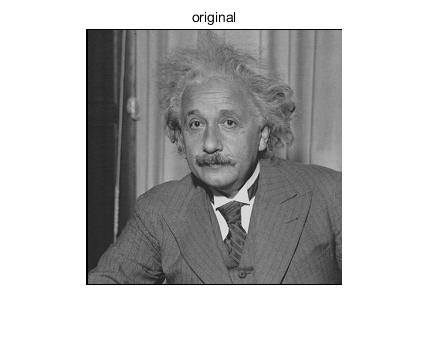
\includegraphics[width=0.45\textwidth]{original.png}}
	\subfigure[Frequenztransforatierles Bild nach Zentrierung]{
		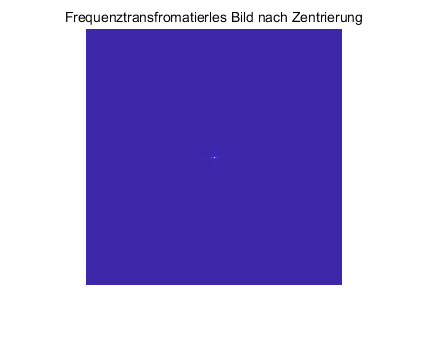
\includegraphics[width=0.45\textwidth]{originalf.png}}
\end{figure*}
\subsection{Ortsraum}
Ein zweidimensionale Faltung erreicht man durch Summation über beide Koordinaten der zweidimensionalen Eingangsfunktion I und des Kerns K. Die Rechnungen lautet:
\begin{equation*}
I'(x,y) = K \cdot I = \sum_{m = -\frac{M-1}{2}}^{\frac{M-1}{2}} \sum_{n = -\frac{N-1}{2}}^{\frac{N-1}{2}} K(m,n) \cdot I(x-m,y-m)
\end{equation*}
wobei $M$ und $N$ sind die Anzahl des Kerns K bzw. des Filters, sie sind normalerweise ungerade Zahlen. In Matlab darf man dieser Schritt mit Funktion 'imfilter' machen. 
\subsection{Frequenzraum}
Die notwendige Transformation der Funktionen zwischen Orts- und Frequenzraum erfolgt durch die Fouriertransformation. Der Filtermaske und der Graph werden mit Fouriertransformation in Frequenzraum geführt und in Bildgröße erweitert. Statt Faltung ist eine Multiplikation zu machen. 
\begin{equation*}
f(x,y) \times h(x,y) \hat{=} F(u,v) \cdot H(u,v)
\end{equation*}
Am Ende wird gefiltetes Bild im Frequenzraum mit inverse Fouriertransformation wieder in den Ortsraum transformiert. 
\newpage
\section{Boxfilter}
Beide Boxfilter und Binomialfilter sind Glättungsfilter, das Rauschen wird geringer aber der Bild wird unschärfer.
\subsection{Ortsraum}
Ein $5 \times 5$ Boxfilter stellt darunter:
\begin{equation*}
\frac{1}{25} \begin{bmatrix}
1 & 1 & 1 & 1 & 1 \\
1 & 1 & 1 & 1 & 1 \\
1 & 1 & 1 & 1 & 1 \\
1 & 1 & 1 & 1 & 1 \\
1 & 1 & 1 & 1 & 1 
\end{bmatrix}
\end{equation*}
Mit der Methode in 1.1
\begin{figure*}[ht]\centering
	\subfigure[Boxfilter in Ortsraum]{
		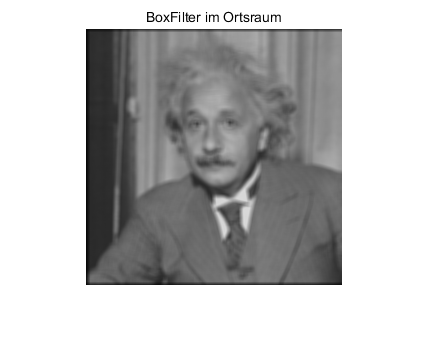
\includegraphics[width=0.45\textwidth]{boxorts.png}}
\end{figure*}
\newpage
\subsection{Frequenzraum}
Filter in Frequenzraum in 2D und 3D Darstellung
\begin{figure*}[ht]\centering
	\subfigure[2D]{
		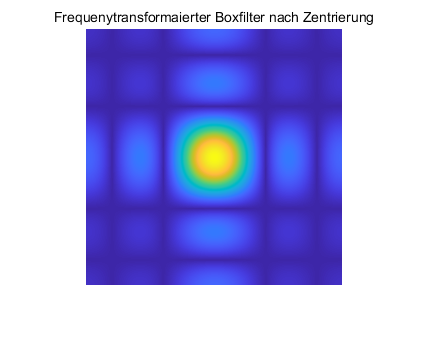
\includegraphics[width=0.45\textwidth]{boxfilter2d.png}}
	\subfigure[3D]{
		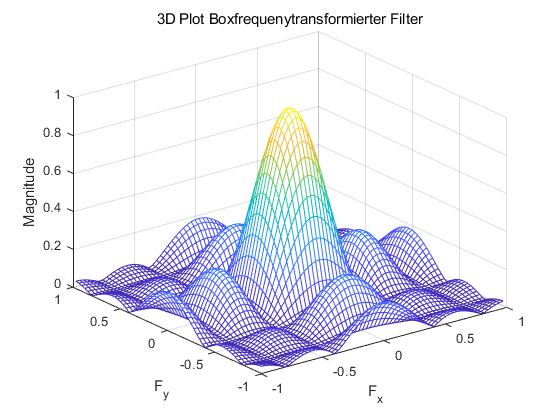
\includegraphics[width=0.45\textwidth]{boxfilter3d.png}}
\end{figure*}
\newline
gefilteter Bild ist heller als in Ortsraum, die Auflösung ist gleich.
\begin{figure*}[ht]\centering
	\subfigure[Boxfilter in Frequenzraum]{
		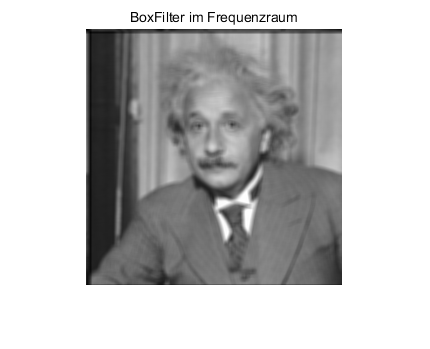
\includegraphics[width=0.45\textwidth]{boxfreq.png}}
\end{figure*}
\section{Binomialfilter}
\subsection{Ortsraum}
$5 \times 5$Maske für Binomialfilterung:
\begin{equation*}
\frac{1}{256} \begin{bmatrix}
1 & 4 & 6 & 4 & 1 \\
4 & 16 & 24 & 16 & 4 \\
6 & 24 & 36 & 24 & 6 \\
4 & 16 & 24 & 16 & 4 \\
1 & 4 & 6 & 4 & 1 
\end{bmatrix}
\end{equation*}
analog: 
\begin{figure*}[ht]\centering
	\subfigure[Binomialfilter in Ortsraum]{
		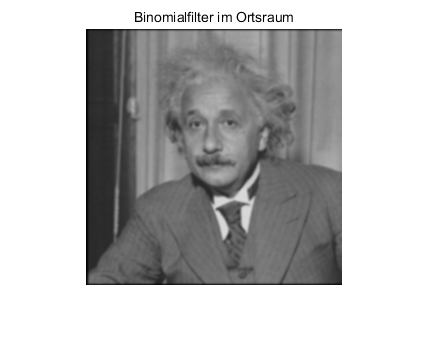
\includegraphics[width=0.45\textwidth]{binoorts.png}}
\end{figure*}
\subsection{Frequenzraum}
Filter in Frequenzraum in 2D und 3D Darstellung
\begin{figure*}[ht]\centering
	\subfigure[2D]{
		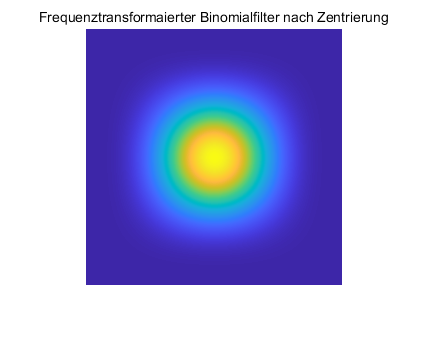
\includegraphics[width=0.45\textwidth]{binofilter2d.png}}
	\subfigure[3D]{
		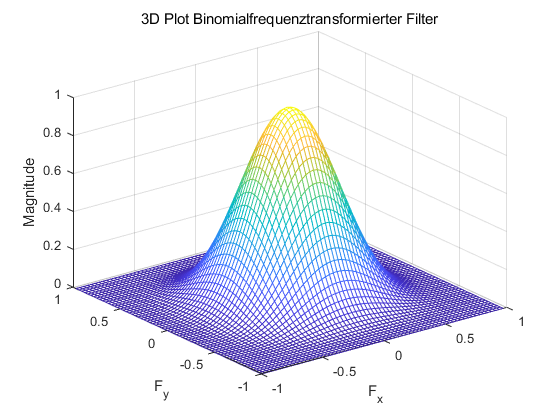
\includegraphics[width=0.45\textwidth]{binofilter3d.png}}
\end{figure*}
\newline
gefilteter Bild ist heller als in Ortsraum, die Auflösung ist gleich.
\begin{figure*}[ht]\centering
	\subfigure[Binomialfilter in Frequenzraum]{
		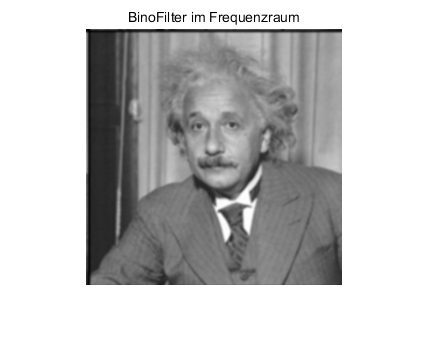
\includegraphics[width=0.45\textwidth]{binofreq.png}}
\end{figure*}
\newpage
\section{Laplace-Filter}
Laplace-Filter und Sobel-Filter werden genutzt durch Kanteverstärkung für Bildverbesserung.
\subsection{Ortsraum}
Maske: 
\begin{equation*}
\begin{bmatrix}
0 & 1 & 0  \\
1 & -4 & 1\\
0 & 1 & 0\\
\end{bmatrix}
\end{equation*}
\begin{figure*}[ht]\centering
	\subfigure[Laplace-Filter in Ortsraum]{
		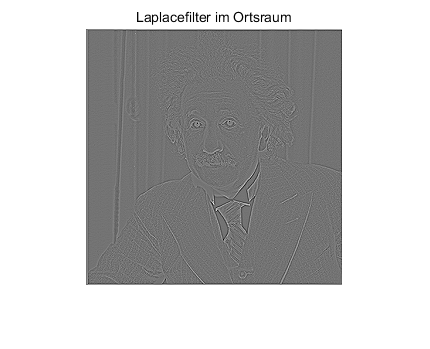
\includegraphics[width=0.45\textwidth]{laplaceorts.png}}
\end{figure*}
\newpage
\subsection{Frequenzraum}
Filter in Frequenzraum in 2D und 3D Darstellung
\begin{figure*}[ht]\centering
	\subfigure[2D]{
		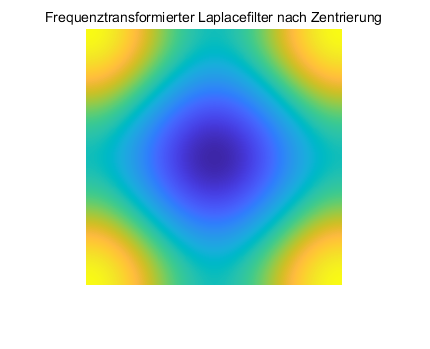
\includegraphics[width=0.45\textwidth]{laplacefilter2d.png}}
	\subfigure[3D]{
		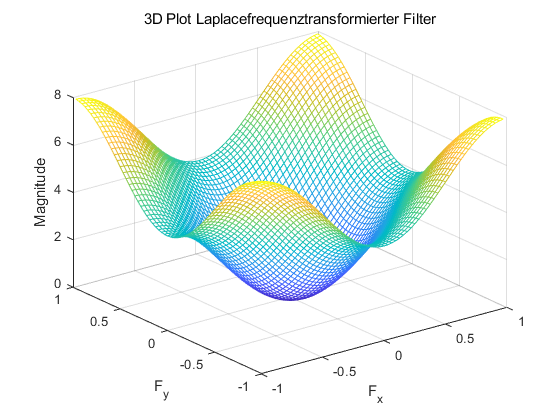
\includegraphics[width=0.45\textwidth]{laplacefilter3d.png}}
\end{figure*}
\newline
gefilteter Bild
\begin{figure*}[ht]\centering
	\subfigure[Laplace-Filter in Frequenzraum]{
		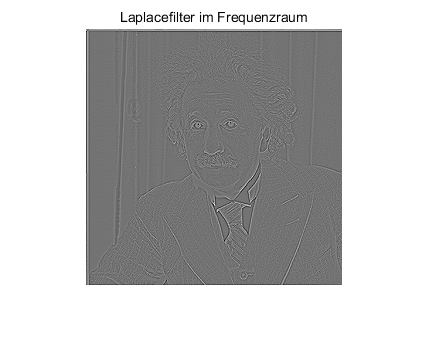
\includegraphics[width=0.45\textwidth]{laplacefreq.png}}
\end{figure*}
\newline
Das Ergebnis sieht gleich wie in Ortsraum
\newpage
\section{Sobel-Filter}
\subsection{Ortsraum}
Maske in x- und y- Richtungen:
\begin{equation*}
\begin{bmatrix}
1 & 0 & -1  \\
2 & 0 & -2\\
1 & 0 & -1\\
\end{bmatrix} \quad 
\begin{bmatrix}
1 & 2 & 1  \\
0 & 0 & 0\\
-1 & -2 & -1\\
\end{bmatrix}
\end{equation*}
\begin{figure*}[ht]\centering
	\subfigure[Sobel x Filter in Ortsraum]{
		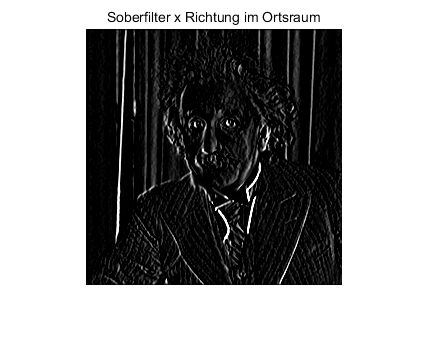
\includegraphics[width=0.3\textwidth]{sobelxorts.png}}
	\subfigure[Sobel y Filter in Ortsraum]{
		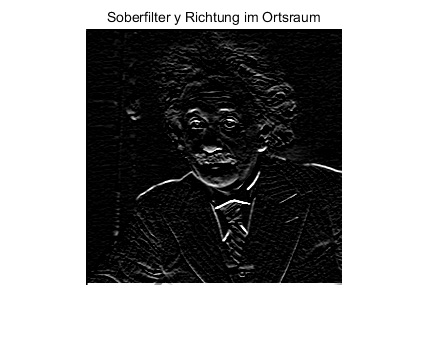
\includegraphics[width=0.3\textwidth]{sobelyorts.png}}
	\subfigure[Gradient in Ortsraum]{
		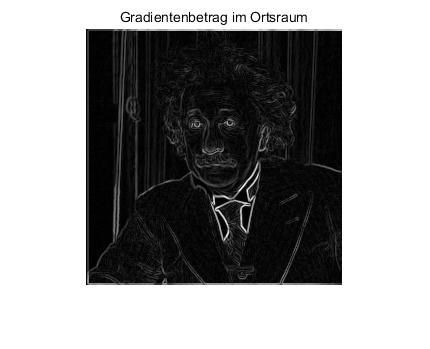
\includegraphics[width=0.3\textwidth]{gradorts.png}}
\end{figure*}
\newpage
\subsection{Frequenzraum}
Filter in Frequenzraum in 2D und 3D Darstellung
\begin{figure*}[ht]\centering
	\subfigure[x 2D]{
		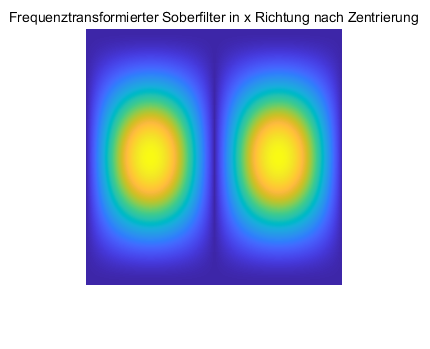
\includegraphics[width=0.45\textwidth]{sobelx2d.png}}
	\subfigure[x 3D]{
		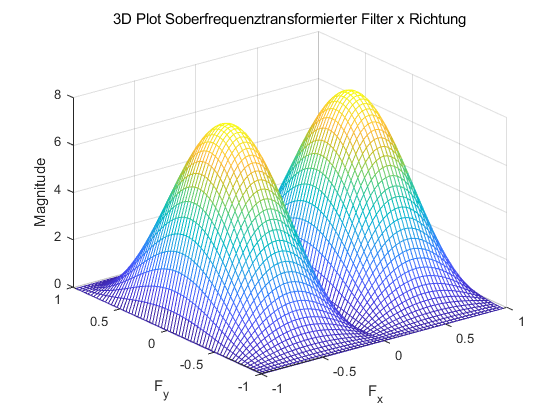
\includegraphics[width=0.45\textwidth]{sobelx3d.png}}
	\subfigure[y 2D]{
		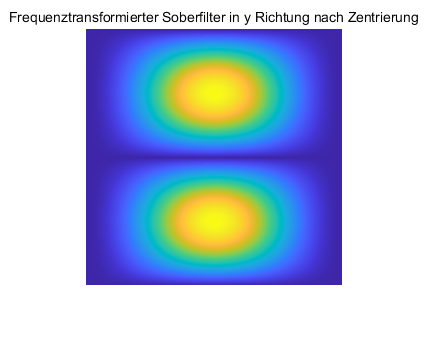
\includegraphics[width=0.45\textwidth]{sobely2d.png}}
	\subfigure[y 3D]{
		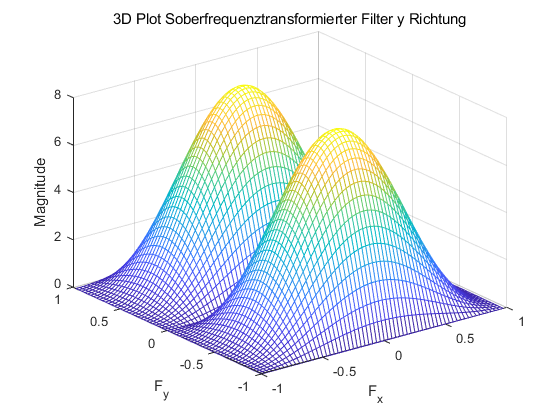
\includegraphics[width=0.45\textwidth]{sobely3d.png}}
\end{figure*}
\newpage
gefilteten Bilden
\begin{figure*}[ht]\centering
	\subfigure[Sobel x Filter in Frequenzraum]{
		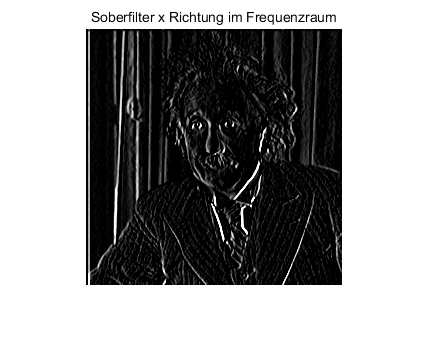
\includegraphics[width=0.3\textwidth]{sobelxfreq.png}}
	\subfigure[Sobel y Filter in Frequenzraum]{
		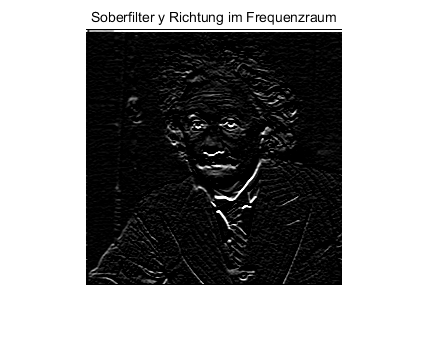
\includegraphics[width=0.3\textwidth]{sobelyfreq.png}}
	\subfigure[Gradient in Frequenzraum]{
		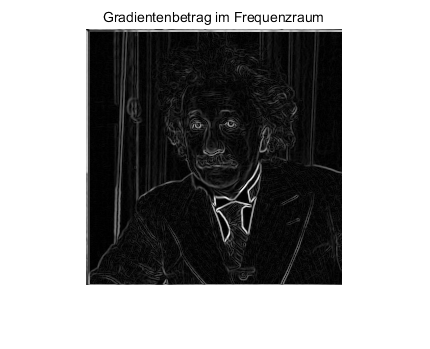
\includegraphics[width=0.3\textwidth]{gradfreq.png}}
\end{figure*}
\newline
Die Ergebnisse sehen gleich wie in Ortsraum
\end{document}